\documentclass[CT4S-EN-RU]{subfiles}

\begin{document}

\section{\caseENGRUS{Finite colimits in $\Set$}{ / }{Конечные копределы в $\Set$}}\label{sec:finite colimits}

\begin{blockENG}
This section will parallel Section \ref{sec:finite limits} — I will introduce several types of finite colimits and hope that this gives the reader some intuition about them, without formally defining them yet. Before doing so, I must define equivalence relations and quotients.
\end{blockENG}

\begin{blockRUS}
Этот раздел воспроизводит структуру Раздела \ref{sec:finite limits} — я ввожу несколько видов конечных копределов в надежде, что это даст читателю интуитивное представление о них, без необходимости их пока формально определять. Однако прежде я введу отношения эквивалентности и фактор-множества.
\end{blockRUS}

%%%% Subsection %%%%

\subsection{\caseENGRUS{Background: equivalence relations}{ / }{Отступление: отношения эквивалентности}}\index{equivalence relation}\index{relation!equivalence}\index{отношение!эквивалентности}

\begin{definitionENG}[Equivalence relations and equivalence classes]
Let $X$ be a set. An {\em equivalence relation on $X$} is a subset $R\ss X\times X$ satisfying the following properties for all $x,y,z\in X$:
\begin{description}
\item[Reflexivity:] $(x,x)\in R$;
\item[Symmetry:] $(x,y)\in R$ if and only if $(y,x)\in R$; and
\item[Transitivity:] if $(x,y)\in R$ and $(y,z)\in R$ then $(x,z)\in R$.
\end{description}
If $R$ is an equivalence relation, we often write $x\sim_R y$, or simply $x\sim y$, to mean $(x,y)\in R$. For convenience we may refer to the equivalence relation by the symbol $\sim$, saying that $\sim$ is an equivalence relation on $X$.\index{a symbol!$\sim$}

An {\em equivalence class of $\sim$}\index{equivalence relation!equivalence classes} is a subset $A\ss X$ such that
\begin{itemize}
\item $A$ is nonempty, $A\neq\emptyset$;
\item if $x\in A$ and $x'\in A$, then $x\sim x'$; and 
\item if $x\in A$ and $x\sim y$, then $y\in A$.
\end{itemize}
Suppose that $\sim$ is an equivalence relation on $X$. The {\em quotient of $X$ by $\sim$}\index{equivalence relation!quotient by}, denoted $X/\sim$\index{a symbol!$X/\sim$} is the set of equivalence classes of $\sim$.
\end{definitionENG}

\begin{definitionRUS}[Отношения эквивалентности и классы эквивалентности]
Пусть $X$ — множество. {\em Отношение эквивалентности на $X$} — это подмножество $R\ss X\times X$, удовлетворяющее следующим условиям для всех $x,y,z\in X$:
\begin{description}
\item[Рефлексивность:] $(x,x)\in R$;
\item[Симметричность:] $(x,y)\in R$ если и только если $(y,x)\in R$; и
\item[Транзитивность:] если $(x,y)\in R$ и $(y,z)\in R$, то $(x,z)\in R$.
\end{description}
Если $R$ — отношение эквивалентности, это часто обозначается $x\sim_R y$ или $x\sim y$, имея в виду $(x,y)\in R$. Для удобства мы, говоря о самом отношении эквивалентности $R$ над $X$, будем обозначать его символом $\sim$.\index{символ!$\sim$}

{\em Классом эквивалентности}\index{equivalence relation!equivalence classes} для $\sim$ называется подмножество $A\ss X$ такое, что
\begin{itemize}
\item $A$ не является пустым, $A\neq\emptyset$;
\item если $x\in A$ и $x'\in A$, то $x\sim x'$; и 
\item если $x\in A$ и $x\sim y$, то $y\in A$.
\end{itemize}
Предположим, что $\sim$ — отношение эквивалентности на $X$. Тогда множество всех классов эквивалентности для $\sim$ называется {\em фактор-множеством $X$ по эквивалентности $\sim$}\index{отношение!эквивалентности!фактор-множество}, обозначаемым $X/\sim$\index{символ!$X/\sim$}.
\end{definitionRUS}

\begin{exampleENG}
Let $\ZZ$ denote the set of integers. Define a relation $R\ss\ZZ\times\ZZ$ by $$R=\{(x,y)\|\exists n\in\ZZ \tn{ such that } x+7n=y\}.$$ Then $R$ is an equivalence relation because $x+7*0=x$ (reflexivity); $x+7*n=y$ if and only if $y+7*(-n)= x$ (symmetry); and $x+7n=y$ and $y+7m=z$ together imply that $x+7(m+n)=z$ (transitivity).
\end{exampleENG}

\begin{exampleRUS}
Пусть $\ZZ$ обозначает множество целых чисел. Определим отношение $R\ss\ZZ\times\ZZ$ таким образом: $$R=\{(x,y)\|\exists n\in\ZZ \tn{ такое, что } x+7n=y\}.$$ Тогда $R$ является отношением эквивалентности, поскольку $x+7*0=x$ (рефлексивность); $x+7*n=y$ если и только если $y+7*(-n)= x$ (симметричность); наконец, из $x+7n=y$ и $y+7m=z$ одновременно следует, что $x+7(m+n)=z$ (транзитивность).
\end{exampleRUS}

\begin{exerciseENG}
Let $X$ be the set of people on earth; define a binary relation $R\ss X\times X$ on $X$ as follows. For a pair $(x,y)$ of people, say $(x,y)\in R$ if $x$ spends a lot of time thinking about $y$. 
\sexc Is this relation reflexive? 
\item Is it symmetric? 
\item Is it transitive?
\endsexc
\end{exerciseENG}

\begin{exerciseRUS}
Пусть $X$ — множество людей на земле; определим бинарное отношение $R\ss X\times X$ на $X$ следующим образом. Для пары людей $(x,y)$ будем считать, что $(x,y)\in R$, если $x$ проводит много времени, думая об $y$. 
\sexc Будет ли это отношение рефлексивным? 
\item Будет ли оно симметричным? 
\item Будет ли оно транзитивным?
\endsexc
\end{exerciseRUS}

\begin{exampleENG}[Partitions]\label{ex:partition}
An equivalence relation on a set $X$ can be thought of as a way of partitioning $X$. A {\em partition of $X$}\index{equivalence relation!as partition} consists of a set $I$, called {\em the set of parts}, and for every element $i\in I$ a subset $X_i\ss X$ such that two properties hold:
\begin{itemize}
\item every element $x\in X$ is in some part (i.e. for all $x\in X$ there exists $i\in I$ such that $x\in X_i$); and
\item no element can be found in two different parts (i.e. if $x\in X_i$ and $x\in X_j$ then $i=j$).
\end{itemize}

Given a partition of $X$, we define an equivalence relation $\sim$ on $X$ by saying $x\sim x'$ if $x$ and $x'$ are in the same part (i.e. if there exists $i\in I$ such that $x,x'\in X_i$). The parts become the equivalence classes of this relation. Conversely, given an equivalence relation, one makes a partition on $X$ by taking $I$ to be the set of equivalence classes and for each $i\in I$ letting $X_i$ be the elements in that equivalence class.
\end{exampleENG}

\begin{exampleRUS}[Разбиения]\label{ex:partition}
Об отношении эквивалентности на множестве $X$ можно думать, как о способе разбить $X$ на части. {\em Разбиение $X$}\index{отношение!эквивалентности!как разбиение} состоит из множества $I$, называемого {\em множеством частей}, и для каждого элемента $i\in I$ — подмножества $X_i\ss X$ такого, что выполняются два условия:
\begin{itemize}
\item каждый элемент $x\in X$ находится в некоторой части (то есть, для всех $x\in X$ существует $i\in I$ такой, что $x\in X_i$); и
\item ни один элемент не находится в двух различных частях (то есть, если $x\in X_i$ и $x\in X_j$, то $i=j$).
\end{itemize}

Для данного рабиения $X$ определим отношение эквивалентности $\sim$ на $X$, положив $x\sim x'$, если $x$ и $x'$ находятся в одной и той же части (то есть, если существует $i\in I$ такой, что $x,x'\in X_i$). Части оказываются классами эквивалентности этого отношения. Обратно, для данного отношения эквивалентности построим разбиение $X$, взяв в качестве $I$ множество классов эквивалентности и для каждого $i\in I$ положив, что $X_i$ состоит из элементов этого класса.
\end{exampleRUS}

\begin{exerciseENG}
Let $X$ and $B$ be sets and let $f\taking X\to B$ be a function. Define a subset $R\ss X\times X$ by $$R=\{(x,y)\|f(x)=f(y)\}.$$ 
\sexc Is $R$ an equivalence relation? 
\item Are all equivalence relations on $X$ obtainable in this way (as the fibers of some function having domain $X$)?
\item Does this viewpoint on equivalence classes relate to that of Example \ref{ex:partition}?
\endsexc
\end{exerciseENG}

\begin{exerciseRUS}
Пусть $X$ и $B$ — это множество, а $f\taking X\to B$ — функция. Определим подмножество $R\ss X\times X$ как $$R=\{(x,y)\|f(x)=f(y)\}.$$ 
\sexc Будет ли $R$ отношением эквивалентности? 
\item Можно ли все отношения эквивалентности на $X$ получить таким же способом (как «слои» некоторой функции с областью определения $X$)?
\item Связана ли эта точка зрения на классы эквивалентности с Примером \ref{ex:partition}?
\endsexc
\end{exerciseRUS}

\begin{exerciseENG}
Take a set $I$ of sets; i.e. suppose that for each element $i\in I$ you are given a set $X_i$. For every two elements $i,j\in I$ say that $i\sim j$ if $X_i$ and $X_j$ are isomorphic. Is this relation an equivalence relation on $I$?  
\end{exerciseENG}

\begin{exerciseRUS}
Возьмем множество $I$ некоторых множеств; то есть предположим, что для каждого элемента $i\in I$ задано множество $X_i$. Для каждых двух элементов $i,j\in I$ будем считать, что $i\sim j$, если $X_i$ и $X_j$ изоморфны. Будет ли это отношение отношением эквивалентности на $I$?
\end{exerciseRUS}

\begin{lemmaENG}[Generating equivalence relations]\label{lemma:generating ERs}
Let $X$ be a set and $R\ss X\times X$ a subset. There exists a relation $S\ss X\times X$ such that
\begin{itemize}
\item $S$ is an equivalence relation,
\item $R\ss S$, and
\item for any equivalence relation $S'$ such that $R\ss S'$, we have $S\ss S'$.
\end{itemize}
The relation $S'$ will be called {\em the equivalence relation generated by $R$}.\index{equivalence relation!generated}
\end{lemmaENG}

\begin{lemmaRUS}[Порождение отношений эквивалентности]\label{lemma:generating ERs}
Пусть $X$ — это множество, а $R\ss X\times X$ — подмножество. Существует отношение $S\ss X\times X$ такое, что
\begin{itemize}
\item $S$ является отношением эквивалентности,
\item $R\ss S$, и
\item для любого отношения эквивалентности $S'$ такого, что $R\ss S'$, выполняется $S\ss S'$.
\end{itemize}
Отношение $S$ назовем {\em отношением эквивалентности, порожденным $R$}.\index{отношение!эквивалентности!порожденное}
\end{lemmaRUS}

\begin{proofENG}
Let $L_R$ be the set of all equivalence relations on $X$ that contain $R$; in other words, each element $\ell\in L_R$ is an equivalence relation, $\ell\in X\times X$. The set $L_R$ is non-empty because $X\times X\ss X\times X$ is an equivalence relation. Let $S$ denote the set of pairs $(x_1,x_2)\in X\times X$ that appear in every element of $L_R$. Note that $R\ss S$ by definition. We need only show that $S$ is an equivalence relation.

It is clearly reflexive, because $R$ is. If $(x,y)\in S$ then $(x,y)\in\ell$ for all $\ell\in L_R$. But since each $\ell$ is an equivalence relation, $(y,x)\in\ell$ too, so $(y,x)\in S$. This shows that $S$ is symmetric. The proof that it is transitive is similar: if $(x,y)\in S$ and $(y,z)\in S$ then they are both in each $\ell$ which puts $(x,z)$ in each $\ell$, which puts it in $S$.
\end{proofENG}

\begin{proofRUS}
Пусть $L_R$ — множество всех отношений эквивалентности на $X$, которые содержат $R$; другими словами, каждый элемент $\ell\in L_R$ будет отношением эквивалентности, $\ell\ss X\times X$. Множество $L_R$ непусто, поскольку $X\times X\ss X\times X$ тоже является отношением эквивалентности. Пусть $S$ обозначает множество пар $(x_1,x_2)\in X\times X$, которые появляются в каждом элементе $L_R$. Заметим, что $R\ss S$ по определению. Нам остается только показать, что $S$ оказывается отношением эквивалентности.

Оно, очевидно, рефлексивно, поскольку этим свойством обладает $R$. Если $(x,y)\in S$, то $(x,y)\in\ell$ для всех $\ell\in L_R$. Но поскольку каждый $\ell$ это отношение эквивалентности, то $(y,x)\in\ell$, а значит, $(y,x)\in S$. Это показывает, что $S$ — симметрично. Доказательство того, что оно транзитивно, аналогично: если $(x,y)\in S$ и $(y,z)\in S$, то они оба принадлежат каждому $\ell$, из чего следует принадлежность $(x,z)$ каждому $\ell$, что, в свою очередь, влечет $(x,z)\in S$.
\end{proofRUS}

\begin{remarkENG}
Let $X$ be a set and $R\ss X\times X$ a relation. The proof of Lemma \ref{lemma:generating ERs} has the benefit of working even if $|X|\geq\infty$, but it has the cost that it is not very intuitive, nor useful in practice when $X$ is finite. The intuitive way to think about the idea of equivalence relation generated by $R$ is as follows.
\begin{enumerate}
\item First add to $R$ what is demanded by reflexivity, $R_1:=R\cup\{(x,x)\|x\in X\}$.
\item Then add to $R$ what is demanded by symmetry, $R_2:=R_1\cup\{(x,y)\|(y,x)\in R_1\}.$
\item Finally, add to $R$ what is demanded by transitivity, $$S=R_2\cup\{(x,z)\|(x,y)\in R_2, \tn{ and } (y,z)\in R_2\}.$$
\end{enumerate}
\end{remarkENG}

\begin{remarkRUS}
Пусть $X$ — множество, а $R\ss X\times X$ — отношение. Доказательство Леммы \ref{lemma:generating ERs} имеет то преимущество, что работает даже для $|X|\geq\infty$, но это достигается за счет того, что оно ни слишком интуитивно, ни полезно на практике, когда $X$ конечно. Интуитивный способ думать об идее отношения эквивалентности, порожденном $R,$ описан ниже.
\begin{enumerate}
\item Прежде всего, добавим к $R$ то, что требуется из-за рефлексивности, $R_1:=R\cup\{(x,x)\|x\in X\}$.
\item Затем добавим к $R$ то, что требуется из-за симмеричности, $R_2:=R_1\cup\{(x,y)\|(y,x)\in R_1\}.$
\item Наконец, добавим к $R$ то, что требуется из-за транзитивности,%
\endnote{Возможно, последний шаг потребуется повторить несколько раз, чтобы учесть цепочки эквивалентностей длиною более $2$.}
$$S=R_2\cup\{(x,z)\|(x,y)\in R_2, \tn{ и } (y,z)\in R_2\}.$$
\end{enumerate}
\end{remarkRUS}

\begin{exerciseENG}
Consider the set $\RR$ of real numbers. Draw the coordinate plane $\RR\times\RR$, give it coordinates $x$ and $y$. A binary relation on $\RR$ is a subset $S\ss\RR\times\RR$, which can be drawn as a set of points in the plane. 
\sexc Draw the relation $\{(x,y)\|y=x^2\}$. 
\item Draw the relation $\{(x,y)\|y\geq x^2\}.$
\item Let $S_0$ be the equivalence relation on $\RR$ generated (in the sense of Lemma \ref{lemma:generating ERs}) by the empty set. Draw $S$ as a subset of the plane.
\item Consider the equivalence relation $S_1$ generated by $\{(1,2),(1,3)\}$. Draw $S_1$ in the plane. Highlight the equivalence class containing $(1,2)$.
\item The reflexivity property and the symmetry property have pleasing visualizations in $\RR\times\RR$; what are they? 
\item Is there a nice heuristic for visualizing the transitivity property?
\endsexc
\end{exerciseENG}

\begin{exerciseRUS}
Рассмотрим множество $\RR$ всех действительных чисел. Изобразим координатную плоскость $\RR\times\RR$ с координатами $x$ и $y$. Бинарное отношение на $\RR$ — это подмножество $S\ss\RR\times\RR$, которое может быть изображено в виде множества точек на нашей плоскости. 
\sexc Изобразите отношение $\{(x,y)\|y=x^2\}$. 
\item Изобразите отношение $\{(x,y)\|y\geq x^2\}.$
\item Пусть $S_0$ — отношение эквивалентности на $\RR$, порожденное (в смысле Леммы \ref{lemma:generating ERs}) пустым множеством. Изобразите $S$ как подмножество плоскости.
\item Рассмотрим отношение эквивалентности $S_1$, порожденное $\{(1,2),(1,3)\}$. Изобразите $S_1$ на плоскости. Выделите класс эквивалентности, содержащий $(1,2)$.\endnote{Какая-то фигня про $(1,2)$, причем во второй редакции еще и с ответом. Класс эквивалентности определяется одним элементом $\RR$ (а не парой) и является подмножеством $\RR$ (а не плоскости).}
\item У свойства рефлексивности и симметричности есть удобная визуализация в $\RR\times\RR$; какая? 
\item Имеется ли хорошая эвристика для визуализации свойства транзитивности?
\endsexc
\end{exerciseRUS}

\begin{exerciseENG}
Consider the binary relation $R=\{(n,n+1)\|n\in\ZZ\}\ss\ZZ\times\ZZ$. 
\sexc What is the equivalence relation generated by $R$? 
\item How many equivalence classes are there?
\endsexc
\end{exerciseENG}

\begin{exerciseRUS}
Рассмотрим бинарное отношение $R=\{(n,n+1)\|n\in\ZZ\}\ss\ZZ\times\ZZ$. 
\sexc Каковы классы эквивалентности, порожденные $R$? 
\item Сколько всего здесь классов эквивалентности?
\endsexc
\end{exerciseRUS}

\begin{exerciseENG}
Suppose $N$ is a network (or graph). Let $X$ be the nodes of the network, and let $R\ss X\times X$ denote the relation such that $(x,y)\in R$ iff there exists an arrow connecting $x$ to $y$.%
\footnote{The word {\em iff} means “if and only if”. In this case we are saying that the pair $(x,y)$ is in $R$ if and only if there exists an arrow connecting $x$ and $y$.\index{iff}}
\sexc What is the equivalence relation $\sim$ generated by $R$? 
\item What is the quotient $X/\sim$?
\endsexc
\end{exerciseENG}

\begin{exerciseRUS}
Предположим, $N$ — это сеть (или граф). Пусть $X$ — узлы сети [или вершины графа], и пусть $R\ss X\times X$ обозначает такое отношение, что $(x,y)\in R$ ттт%
\footnote{Слово {\em ттт}\index{ттт} означает «тогда и только тогда, когда». В данном случае мы говорим, что пара $(x,y)$ принадлежит $R$, если и только если существует стрелка, соединяющая $x$ с $y$.}
существует стрелка, соединяющая $x$ с $y$.
\sexc Каково отношение эквивалентности $\sim$, порожденное $R$? 
\item Каким будет фактор-множество $X/\sim$?
\endsexc
\end{exerciseRUS}

%%%% Subsection %%%%

\subsection{\caseENGRUS{Pushouts}{ / }{Пушауты и выталкивающие квадраты}}\label{sec:pushouts}

\begin{definitionENG}[Pushout]\label{def:pushout}
Suppose given the diagram of sets and functions below:
\begin{align}\label{dia:pushout}
\xymatrix{W\ar[r]^f\ar[d]_g&X\\Y}
\end{align}
Its {\em fiber sum},\index{fiber sum} denoted $X\sqcup_WY$, is defined as the quotient of $X\sqcup W\sqcup Y$ by the equivalence relation $\sim$ generated by $w\sim f(w)$ and $w\sim g(w)$ for all $w\in W$.
$$X\sqcup_WY:=(X\sqcup W\sqcup Y)/\sim \hsp\tn{where } \forall w\in W,\;\;  w\sim f(w)\;\;\tn{ and }\;\; w\sim g(w).$$ 
There are obvious inclusions $i_1\taking X\to X\sqcup_WY$ and $i_2\taking Y\to X\sqcup_WY$.%
\footnote{Note that our term inclusions is not too good, because it seems to suggest that $i_1$ and $i_2$ are injective (see Definition \ref{def:inj,surj,bij}) and this is not always the case.}
Note that if $Z=X\sqcup_WY$ then the diagram
\begin{align}\label{dia:pushout sets}
\xymatrix{W\ar[r]^g\ar[d]_f&Y\ar[d]^{i_2}\\X\ar[r]_-{i_1}&Z\lrlimit}
\end{align} 
commutes. Given the setup of Diagram \ref{dia:pushout} we define the {\em pushout of $X$ and $Y$ over $W$} to be any set $Z$ for which we have an isomorphism $Z\To{\iso}X\sqcup_WY$. The corner symbol $\ulcorner$ in Diagram \ref{dia:pushout sets} indicates that $Z$ is the pushout.\index{a symbol!$\ulcorner$}
\end{definitionENG}

\begin{definitionRUS}[Выталкивающий квадрат]\label{def:pushout}
Предположим, дана следующая диаграмма множеств и функций:
\begin{align}\label{dia:pushout}
\xymatrix{W\ar[r]^f\ar[d]_g&X\\Y}
\end{align}
Ее {\em связная сумма},\index{связная сумма} обозначаемая $X\sqcup_WY$, определяется как фактор-множество $X\sqcup W\sqcup Y$ по отношению эквивалентности $\sim$, порожденному $w\sim f(w)$ и $w\sim g(w)$ для всех $w\in W$.
$$X\sqcup_WY:=(X\sqcup W\sqcup Y)/\sim \hsp\tn{где } \forall w\in W,\;\;  w\sim f(w)\;\;\tn{ и }\;\; w\sim g(w).$$ 
Имеются очевидные вложения  $i_1\taking X\to X\sqcup_WY$  и  $i_2\taking Y\to X\sqcup_WY$.%
\footnote{Заметим, что наш термин вложения не особенно подходит, поскольку может показаться, что он предполагает, будто $i_1$ и $i_2$ инъективны (см. Определение \ref{def:inj,surj,bij}), а это не всегда так.}
Заметим, что если $Z=X\sqcup_WY$, то диаграмма
\begin{align}\label{dia:pushout sets}
\xymatrix{W\ar[r]^g\ar[d]_f&Y\ar[d]^{i_2}\\X\ar[r]_-{i_1}&Z\lrlimit}
\end{align} 
коммутирует. Для данной Диаграммы \ref{dia:pushout} мы определим {\em пушаут $X$ и $Y$ над $W$} как произвольное множество $Z$, для которого имеется изоморфизм $Z\To{\iso}X\sqcup_WY$. Символ-уголок $\ulcorner$ в Диаграмме \ref{dia:pushout sets} означает, что $Z$ является пушаутом.\index{символ!$\ulcorner$} [Саму эту диаграмму мы будем называть {\em выталкивающим квадратом}\index{выталкивающий квадрат}, аналогично двойственному случаю введенных ранее притягивающих квадратов.]
\end{definitionRUS}

\begin{exampleENG}
Let $X=\{x\in\RR\|0\leq x\leq1\}$ be the set of numbers between 0 and 1, inclusive, let $Y=\{y\in\RR\|1\leq y\leq 2\}$ by the set of numbers between 1 and 2, inclusive, and let $W=\{1\}$. Then the pushout $X\From{f} W\To{g} Y$, where $f$ and $g$ are the “obvious” functions ($1\mapsto 1$) is $X\sqcup_WY\iso\{z\in\RR\|0\leq z\leq 2\}$, as expected. When we eventually get to general colimits, one can check that the whole real line can be made by patching together intervals in this way.
\end{exampleENG}

\begin{exampleRUS}
Пусть $X=\{x\in\RR\|0\leq x\leq1\}$ — это множество [действительных] чисел от 0 до 1 включительно, $Y=\{y\in\RR\|1\leq y\leq 2\}$ — множество чисел от 1 до 2 включительно и, наконец, $W=\{1\}$. Тогда пушаутом $X\From{f} W\To{g} Y$, где $f$ и $g$ — «очевидные» функции ($1\mapsto 1$), оказывается $X\sqcup_WY\iso\{z\in\RR\|0\leq z\leq 2\}$, как и можно было ожидать. Когда мы доберемся к общему понятию пределов, можно будет убедиться, что при сшивании отдельных интервалов аналогичным образом получается целиком вся действительная прямая.
\end{exampleRUS}

\begin{exampleENG}[Pushout]\label{ex:pushout}
In each example below, the diagram to the right is intended to be a pushout of the diagram to the left.  The new object, $D$, is the union of $B$ and $C$, but instances of $A$ are equated to their $B$ and $C$ aspects.  This will be discussed after the two diagrams.

\begin{align}
\label{dia:po1}\fbox{\xymatrixnocompile{\obox{A}{.7in}{a cell in the shoulder}\LA{r}{is}\LAL{d}{is}&\obox{C}{.6in}{a cell in the arm}\\\obox{B}{.7in}{a cell in the torso}}}\hsp&\fbox{\xymatrix{\obox{A}{.7in}{a cell in the shoulder}\LA{r}{is}\LAL{d}{is}&\obox{C}{.6in}{a cell in the arm}\LA{d}{}\\\obox{B}{.7in}{a cell in the torso}\LA{r}{}&\obox{D=B\sqcup_AC}{.8in}{a cell in the torso or arm}}}
\end{align}
In the left-hand olog (\ref{dia:po1}, the two arrows are inclusions: the author considers every cell in the shoulder to be both in the arm and in the torso. The pushout is then just the union, where cells in the shoulder are not double-counted.

\begin{align}\label{dia:po2}\fbox{\xymatrixnocompile@=18pt{\obox{A}{.8in}{\rr a college mathematics course}\LA{r}{yields}\LAL{d}{is}&\obox{C}{.8in}{an utterance of the phrase “too hard”}\\\obox{B}{.6in}{\rr a college course}}}\hsp&\fbox{\xymatrixnocompile@=18pt{\obox{A}{.8in}{\rr a college mathematics course}\LA{r}{yields}\LAL{d}{is}&\obox{C}{.8in}{an utterance of the phrase “too hard”}\LA{d}{}\\\obox{B}{.6in}{\rr a college course}\LA{r}{}&\obox{\parbox{.6in}{\vspace{.1in}\tiny$D=B\!\sqcup_A\!C$}}{1in}{\rr a college course, where every mathematics course is replaced by an utterance of the phrase “too hard”}}}
\end{align}

In Olog (\ref{dia:po1}), the shoulder is seen as part of the arm and part of the torso.  When taking the union of these two parts, we do not want to “double-count” the shoulder (as would be done in the coproduct $B\sqcup C$, see Example \ref{ex:coproduct2}).  Thus we create a new type $A$ for cells in the shoulder, which are considered the same whether viewed as cells in the arm or cells in the torso.  In general, if one wishes to take two things and glue them together, with $A$ as the glue and with $B$ and $C$ as the two things to be glued, the union is the pushout $B\sqcup_AC$. (A nice image of this can be seen in the setting of topological spaces, see Example \ref{ex:pushout in Top}.)

In Olog (\ref{dia:po2}), if every mathematics course is simply “too hard,” then when reading off a list of courses, each math course will not be read aloud but simply read as “too hard.”  To form $D$ we begin by taking the union of $B$ and $C$, and then we consider everything in $A$ to be the same whether one looks at it as a course or as the phrase “too hard.”  The math courses are all blurred together as one thing.  Thus we see that the power to equate different things can be exercised with pushouts.
\end{exampleENG}

\begin{exampleRUS}[Выталкивающие квадраты]\label{ex:pushout}
В каждом примере ниже, диаграмма справа должна быть выталкивающим квадратом диаграммы слева.  То есть новый тип $D$ является объединением типов $B$ и $C$, при этом экземпляры $A$ считаются совпадающими со своими аспектами в $B$ и $C$.  Под диаграммами мы обсудим это [более подробно].

\begin{align}
\label{dia:po1}\fbox{\xymatrixnocompile{\obox{A}{.7in}{клетка в плече}\LA{r}{это}\LAL{d}{это}&\obox{C}{.6in}{клетка в руке}\\\obox{B}{.7in}{клетка в туловище}}}\hsp&\fbox{\xymatrix{\obox{A}{.7in}{клетка в плече}\LA{r}{это}\LAL{d}{это}&\obox{C}{.6in}{клетка в руке}\LA{d}{}\\\obox{B}{.7in}{клетка в туловище}\LA{r}{}&\obox{D=B\sqcup_AC}{.8in}{клетка в туловище или в руке}}}
\end{align}
На ологе слева (\ref{dia:po1}), две стрелки — это вложения: автор рассматривает каждую клетку в плече как принадлежащую одновременно руке и туловищу. Пушаут тогда является обычным объединением, в котором мы не учитываем клетки в плече дважды.%
\endnote{
Более общо, конструкция объединения множеств из классической теории множеств реализуется средствами теории категорий аналогичным способом как выталкивающий квадрат.
}

В ологе (\ref{dia:po1}) плечо рассматривается как часть руки и одновременно как часть туловища. Образуя объединение этих двух частей, мы не хотим получить продублированное плечо (как получилось бы в случае копроизведения $B\sqcup C$, см. Пример \ref{ex:coproduct2}). Поэтому мы описали новый тип $A$ для клеток плеча, которые считаются одними и теми же, и в качестве клеток плеча, и как клетки туловища. В общем случае, если требуется взять две вещи и склеить их вместе, считая $A$ клеем, а $B$ и $C$ — склеиваемыми вещами, то объединение будет пушаутом $B\sqcup_AC$. (Хорошую иллюстрацию этого можно увидеть в случае топологических пространств, см. Пример \ref{ex:pushout in Top}.)

\begin{align}\label{dia:po2}\fbox{\xymatrixnocompile@=20pt{\obox{A}{1in}{\rr математический предмет в колледже}\LA{r}{\scriptsize вызывает}\LAL{d}{это}&\obox{C}{.8in}{фраза «слишком сложно»}\\\obox{B}{.6in}{\rr предмет в колледже}}}\hsp&\fbox{\xymatrixnocompile@=16pt{\obox{A}{1in}{\rr математический предмет в колледже}\LA{r}{\scriptsize вызывает}\LAL{d}{это}&\obox{C}{.8in}{фраза «слишком сложно»}\LA{d}{}\\\obox{B}{.6in}{\rr предмет в колледже}\LA{r}{}&\obox{\parbox{.6in}{\vspace{.1in}\scriptsize$D=B\!\sqcup_A\!C$}}{1.2in}{\rr предмет в колледже (математические предметы заменены фразой «слишком сложно»)}}}
\end{align}

В ологе (\ref{dia:po2}), если каждый математический предмет просто «слишком сложен,» то при зачитывании подряд всего списка предметов каждый математический предмет не будет зачитан вслух, а просто будет произнесено «слишком сложен.»  Чтобы получить $D$, мы начнем с простого объединения $B$ и $C$, а затем станем считать все в $A$ одним и тем же, смотрим ли мы на предмет или на фразу «слишком сложен.»  В результате все математические предметы смешиваются вместе в одну вещь.  Таким образом мы видим, что в умении приравнивать между собой различные вещи можно тренироваться на пушаутах.
\end{exampleRUS}

\begin{exerciseENG}
Let $W,X,Y$ be as drawn and $f\taking W\to X$ and $g\taking W\to Y$ the indicated functions. 
\begin{center}
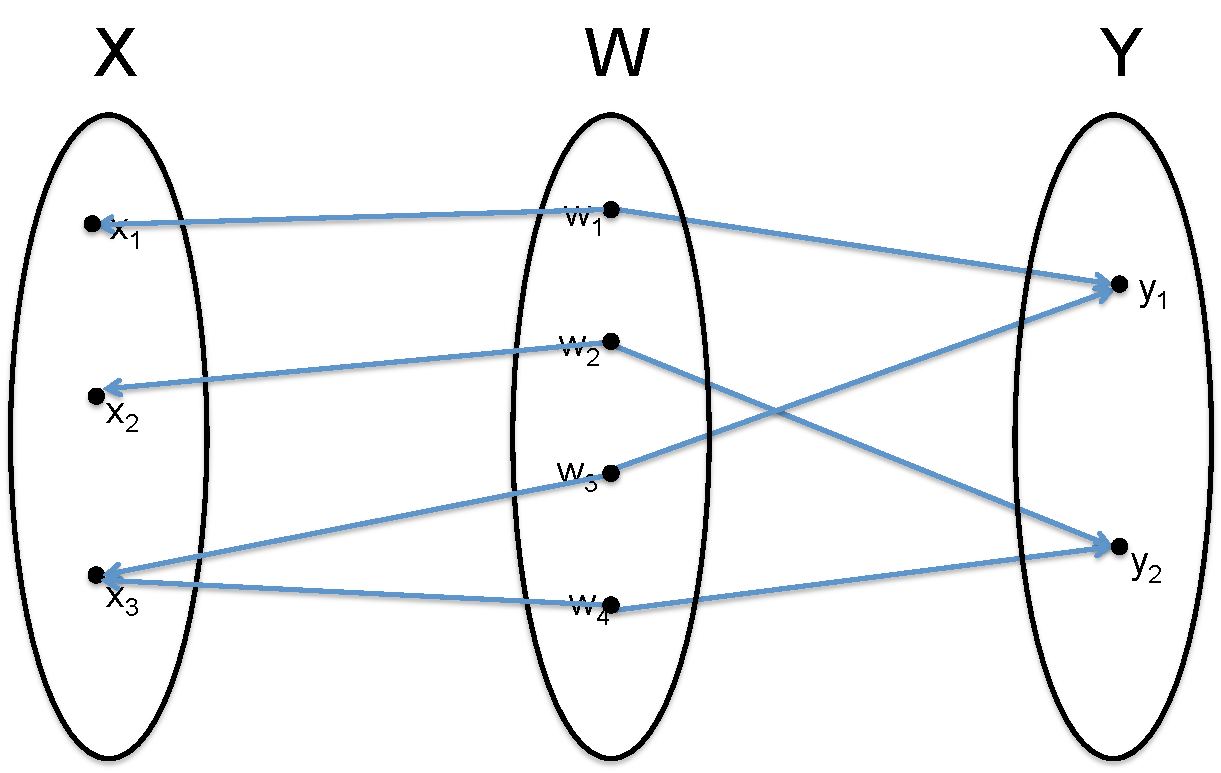
\includegraphics[height=2in]{setPushout}
\end{center}
The pushout of the diagram $X\Fromm{f}W\Too{g}Y$ is a set $P$. Write down the cardinality of $P\iso\ul{n}$ as a natural number $n\in\NN$.  
\end{exerciseENG}

\begin{exerciseRUS}
Пусть множества $W,X,Y$ и функции $f\taking W\to X$ и $g\taking W\to Y$ такие, как изображено ниже . 
\begin{center}
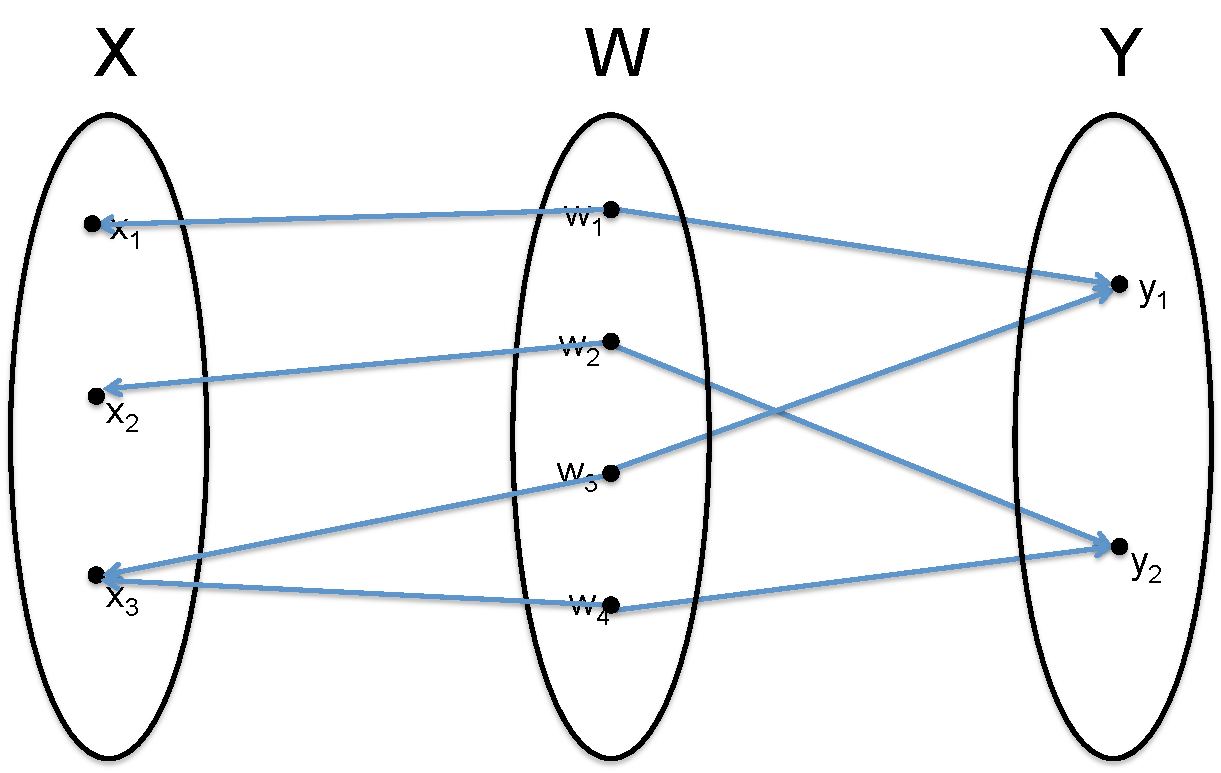
\includegraphics[height=2in]{setPushout}
\end{center}
Пушаут диаграммы $X\Fromm{f}W\Too{g}Y$ это множество $P$. Запишите мощность $P\iso\ul{n}$ в виде натурального числа $n\in\NN$.  
\end{exerciseRUS}

\begin{exerciseENG}
Suppose that $W=\emptyset$; what can you say about $X\sqcup_WZ$? 
\end{exerciseENG}

\begin{exerciseRUS}
Предположим, что $W=\varnothing$; что вы можете сказать о $X\sqcup_WZ$? 
\end{exerciseRUS}

\begin{exerciseENG}
Let $W:=\NN=\{0,1,2,\ldots\}$ denote the set of natural numbers, let $X=\ZZ$ denote the set of integers, and let $Y=\singleton$ denote a one-element set. Define $f\taking W\to X$ by $f(w)= -(w+1)$, and define $g\taking W\to Y$ to be the unique map. Describe the set $X\sqcup_WY$.
\end{exerciseENG}

\begin{exerciseRUS}
Пусть $W:=\NN=\{0,1,2,\ldots\}$ обозначает множество всех натуральных чисел, $X=\ZZ$ — можество всех целых чисел, и $Y=\singleton$ — одноэлементное множество. Определим $f\taking W\to X$ как $f(w)= -(w+1)$, и $g\taking W\to Y$ как единственное отображение такого вида. Опишите множество $X\sqcup_WY$.
\end{exerciseRUS}

\begin{exerciseENG}
Let $i\taking R\ss X\times X$ be an equivalence relation (see Example \ref{ex:subset as function} for notation). Composing with the projections $\pi_1,\pi_2\taking X\times X\to X$, we have two maps $\pi_1\circ i,\taking R\to X$ and $\pi_2\circ i\taking R\to X$. 
\sexc What is the pushout $$X\From{\pi_1\circ i}R\To{\pi_2\circ i}X?$$ 
\item If $i\taking R\ss X\times X$ is not assumed to be an equivalence relation, we can still define the pushout above. Is there a relationship between the pushout $X\From{\pi_1\circ i}R\To{\pi_2\circ i}X$ and the equivalence relation generated by $R\ss X\times X$?
\endsexc
\end{exerciseENG}

\begin{exerciseRUS}
Пусть $i\taking R\ss X\times X$ — это отношение эквивалентности (про обозначения см. Пример \ref{ex:subset as function}). Беря композицию с проекциями $\pi_1,\pi_2\taking X\times X\to X$, получим два отображения $\pi_1\circ i\taking R\to X$ и $\pi_2\circ i\taking R\to X$. 
\sexc Каким будет пушаут $$X\From{\pi_1\circ i}R\To{\pi_2\circ i}X?$$ 
\item Даже если $i\taking R\ss X\times X$ не обязательно отношение эквивалентности, мы все равно можем определить такой пушаут, как выше. Имеется ли связь между пушаутом $X\From{\pi_1\circ i}R\To{\pi_2\circ i}X$ и отношением эквивалентности, порожденным $R\ss X\times X$?
\endsexc
\end{exerciseRUS}

\begin{lemmaENG}[Universal property for pushout]\label{lemma:up for po}
Suppose given the diagram of sets and functions as below.
\begin{align*}
\xymatrix{W\ar[r]^u\ar[d]_t&Y\\
X}
\end{align*}
For any set $A$ and commutative solid arrow diagram as below (i.e. functions $f\taking X\to A$ and $g\taking Y\to A$ such that $f\circ t=g\circ u$), 
\begin{align}\label{dia:universal property of po}
\xymatrix{
&W\ar[dr]^u\ar[dl]_t\\
X\ar@/_1pc/[dddr]_{i_1}\ar[rd]_f&&Y\ar@/^1pc/[dddl]^{i_2}\ar[dl]^g\\
&A\\\\
&X\sqcup_WY\ar@{-->}[uu]^{\exists!}
}
\end{align}
there exists a unique arrow $\po{f}{g}{W}\taking X\sqcup_WY\to A$ making everything commute, $$f=\po{f}{g}{W}\circ i_1\hsp\text{and}\hsp g=\po{f}{g}{W}\circ i_2.$$
\end{lemmaENG}

\begin{lemmaRUS}[Универсальное свойство выталкивающего квадрата]\label{lemma:up for po}
Предположим, дана такая диаграмма множеств и функций, как ниже.
\begin{align*}
\xymatrix{W\ar[r]^u\ar[d]_t&Y\\
X}
\end{align*}
Для любого множества $A$ и коммутативной диаграммы (из сплошных стрелок) ниже (то есть функций $f\taking X\to A$ и $g\taking Y\to A$ таких, что $f\circ t=g\circ u$), 
\begin{align}\label{dia:universal property of po}
\xymatrix{
&W\ar[dr]^u\ar[dl]_t\\
X\ar@/_1pc/[dddr]_{i_1}\ar[rd]_f&&Y\ar@/^1pc/[dddl]^{i_2}\ar[dl]^g\\
&A\\\\
&X\sqcup_WY\ar@{-->}[uu]^{\exists!}
}
\end{align}
существует единственная стрелка $\po{f}{g}{W}\taking X\sqcup_WY\to A$, делающая коммутативной всю диаграмму, $$f=\po{f}{g}{W}\circ i_1\hsp\text{ и }\hsp g=\po{f}{g}{W}\circ i_2.$$
\end{lemmaRUS}

%%%% Subsection %%%%

\subsection{\caseENGRUS{Other finite colimits}{ / }{Другие конечные копределы}}

\begin{definitionENG}[Coequalizer]\index{coequalizer}\label{def:coequalizer}
Suppose given two parallel arrows 
\begin{align}\label{dia:coequalizer}
\xymatrix{X\ar@<.5ex>[r]^f\ar@<-.5ex>[r]_g&Y.}\hspace{1in}\xymatrix{X\ar@<.5ex>[r]^f\ar@<-.5ex>[r]_g&Y\ar[r]^-q&Coeq(f,g)}
\end{align}
The {\em coequalizer of $f$ and $g$} is the commutative diagram as to the right in (\ref{dia:coequalizer}), where we define $$Coeq(f,g):=Y\;/\;f(x)\sim g(x)$$ i.e. the coequalizer of $f$ and $g$ is the quotient of $Y$ by the equivalence relation generated by $\{(f(x),g(x))\|x\in X\}\ss Y\times Y$
\end{definitionENG}

\begin{definitionRUS}[Коуравнитель]\index{коуравнитель}\label{def:coequalizer}
Предположим, даны две параллельные стрелки 
\begin{align}\label{dia:coequalizer}
\xymatrix{X\ar@<.5ex>[r]^f\ar@<-.5ex>[r]_g&Y}\hspace{1in}\xymatrix{X\ar@<.5ex>[r]^f\ar@<-.5ex>[r]_g&Y\ar[r]^-q&Coeq(f,g).}
\end{align}
{\em Коуравнитель $f$ и $g$} — это коммутативная диаграмма справа (\ref{dia:coequalizer}), где мы определили $$Coeq(f,g):=Y\;/\;f(x)\sim g(x)$$ т.е. коуравнитель $f$ и $g$ совпадает с фактор-множеством $Y$ по отношению эквивалентности, порожденному $\{(f(x),g(x))\|x\in X\}\ss Y\times Y.$
\end{definitionRUS}

\begin{exerciseENG}
Let $X=\RR$ be the set of real numbers. What is the coequalizer of the two maps $X\to X$ given by $x\mapsto x$ and $x\mapsto (x+1)$ respectively?
\end{exerciseENG}

\begin{exerciseRUS}
Пусть $X=\RR$ — множество всех действительных чисел. Каким будет коуравнитель двух отображений $X\to X$, заданных как $x\mapsto x$ и $x\mapsto (x+1)$ соответственно?
\end{exerciseRUS}

\begin{exerciseENG}
Find a universal property enjoyed by the coequalizer of two arrows.
\end{exerciseENG}

\begin{exerciseRUS}
Придумайте универсальное свойство, которым обладает коуравнитель двух стрелок.
\end{exerciseRUS}

\begin{exerciseENG}[Initial object]\label{exc:initial set}
An initial set is a set $S$ such that for every set $A$, there exists a unique function $S\to A$. 
\sexc Find an initial set. 
\item Do you think that the notion {\em initial set} belongs in this section (Section \ref{sec:finite colimits})? How so? If coproducts, pushouts, and coequalizers are all colimits, what do colimits have in common?
\endsexc
\end{exerciseENG}

\begin{exerciseRUS}[Инициальный объект]\label{exc:initial set}
Инициальное множество — это множество $S$ такое, что для каждого множества $A$ существует единственная функция $S\to A$. 
\sexc Найдите инициальное множество. 
\item Как вы думаете, должно ли понятие {\em инициального множества} принадлежать данному разделу (Раздел \ref{sec:finite colimits})? Почему? Если копроизведения, пушауты и коуравнители являются одновременно копределами, то что общего имеют все копределы?
\endsexc
\end{exerciseRUS}

\end{document}
